%%%%%%%%%%%%%%%%%%%%%%%%%%%%%%%%%%%%%%%%%%%%%%%%%%%%%%%%%%%%%%%%%%%%%%%%%%%%%%%%
%2345678901234567890123456789012345678901234567890123456789012345678901234567890
%        1         2         3         4         5         6         7         8
% THESIS CHAPTER

\chapter{Examined algorithms}
\label{chap:algorithms}
\ifpdf
    \graphicspath{{Algorithms/Figures/PNG/}{EvaluationTask/Figures/PDF/}{Algorithms/Figures/}}
\else
    \graphicspath{{Algorithms/Figures/EPS/}{EvaluationTask/Figures/}}
\fi


% short summary of the chapter
The main algorithms analysed in the project are attempted to be as different as
possible from each other. This allows covering as many audio features and
similarity measuring techniques as possible. My motivations of the choice of
algorithms were influenced by the study on MIREX submissions, as well as the
overall scope of features they encompass. 

Julien Osmalsky coins the term \textit{rejector} to define a pairwise comparison
function that given two audio tracks it returns a score ranking of similarity
between both tracks \cite{osmalsky2015combining}. This term was adopted by the
project to refer to each of the algorithms examined. The relation between an
algorithm paper and its rejector term is outlined in section \ref{sec:algolist}.

The final selection includes 5 individual algorithms and an algorithm
aggregating results from 4 of them. Each of the algorithms is examined
individually, with the results from some of them combined through the rank
aggregation algorithm. A lot of the algorithm details are deduced based on
related literature or past papers written by the academics who created the algorithm.

Any implementation information about an algorithm is either taken from the
algorithm paper or through my own experimentation and research.

\section{Algorithms list}
\label{sec:algolist}
The analysis if performed on the following algorithm:
\begin{itemize}
    \item \textbf{Weak rejector} - Osmalskyj, Julien, Marc Van Droogenbroeck,
    and Jean-Jacques Embrechts. \textit{Enhancing cover song identification with
    hierarchical rank aggregation} \cite{osmalsky2016enhancing}
    \item \textbf{Cross-correlation rejector} - Ellis, Daniel PW, Courtenay V.
    Cotton, and Michael I. Mandel. \textit{Cross-correlation of beat-synchronous
    representations for music similarity} \cite{ellis2008cross}
    \item \textbf{Quantisation rejector} - Osmalskyj, Julien, et al.
    \textit{Combining features for cover song identification} \cite{osmalsky2015combining}
    \item \textbf{Timbre rejector} - Tralie, Christopher J., and Paul Bendich.
    \textit{Cover song identification with timbral shape sequences} \cite{tralie2015cover}
    \item \textbf{Aggregated rank rejector} - Osmalskyj, Julien, Marc Van
    Droogenbroeck, and Jean-Jacques Embrechts. \textit{Enhancing cover song
    identification with hierarchical rank aggregation}
    \cite{osmalsky2016enhancing} 
    \item \textbf{Fingerprint rejector} - Rafii, Zafar, Bob Coover, and Jinyu
    Han. \textit{An audio fingerprinting system for live version identification
    using image processing techniques} \cite{rafii2014audio}
\end{itemize}

\begin{figure}[H]
    \centering
    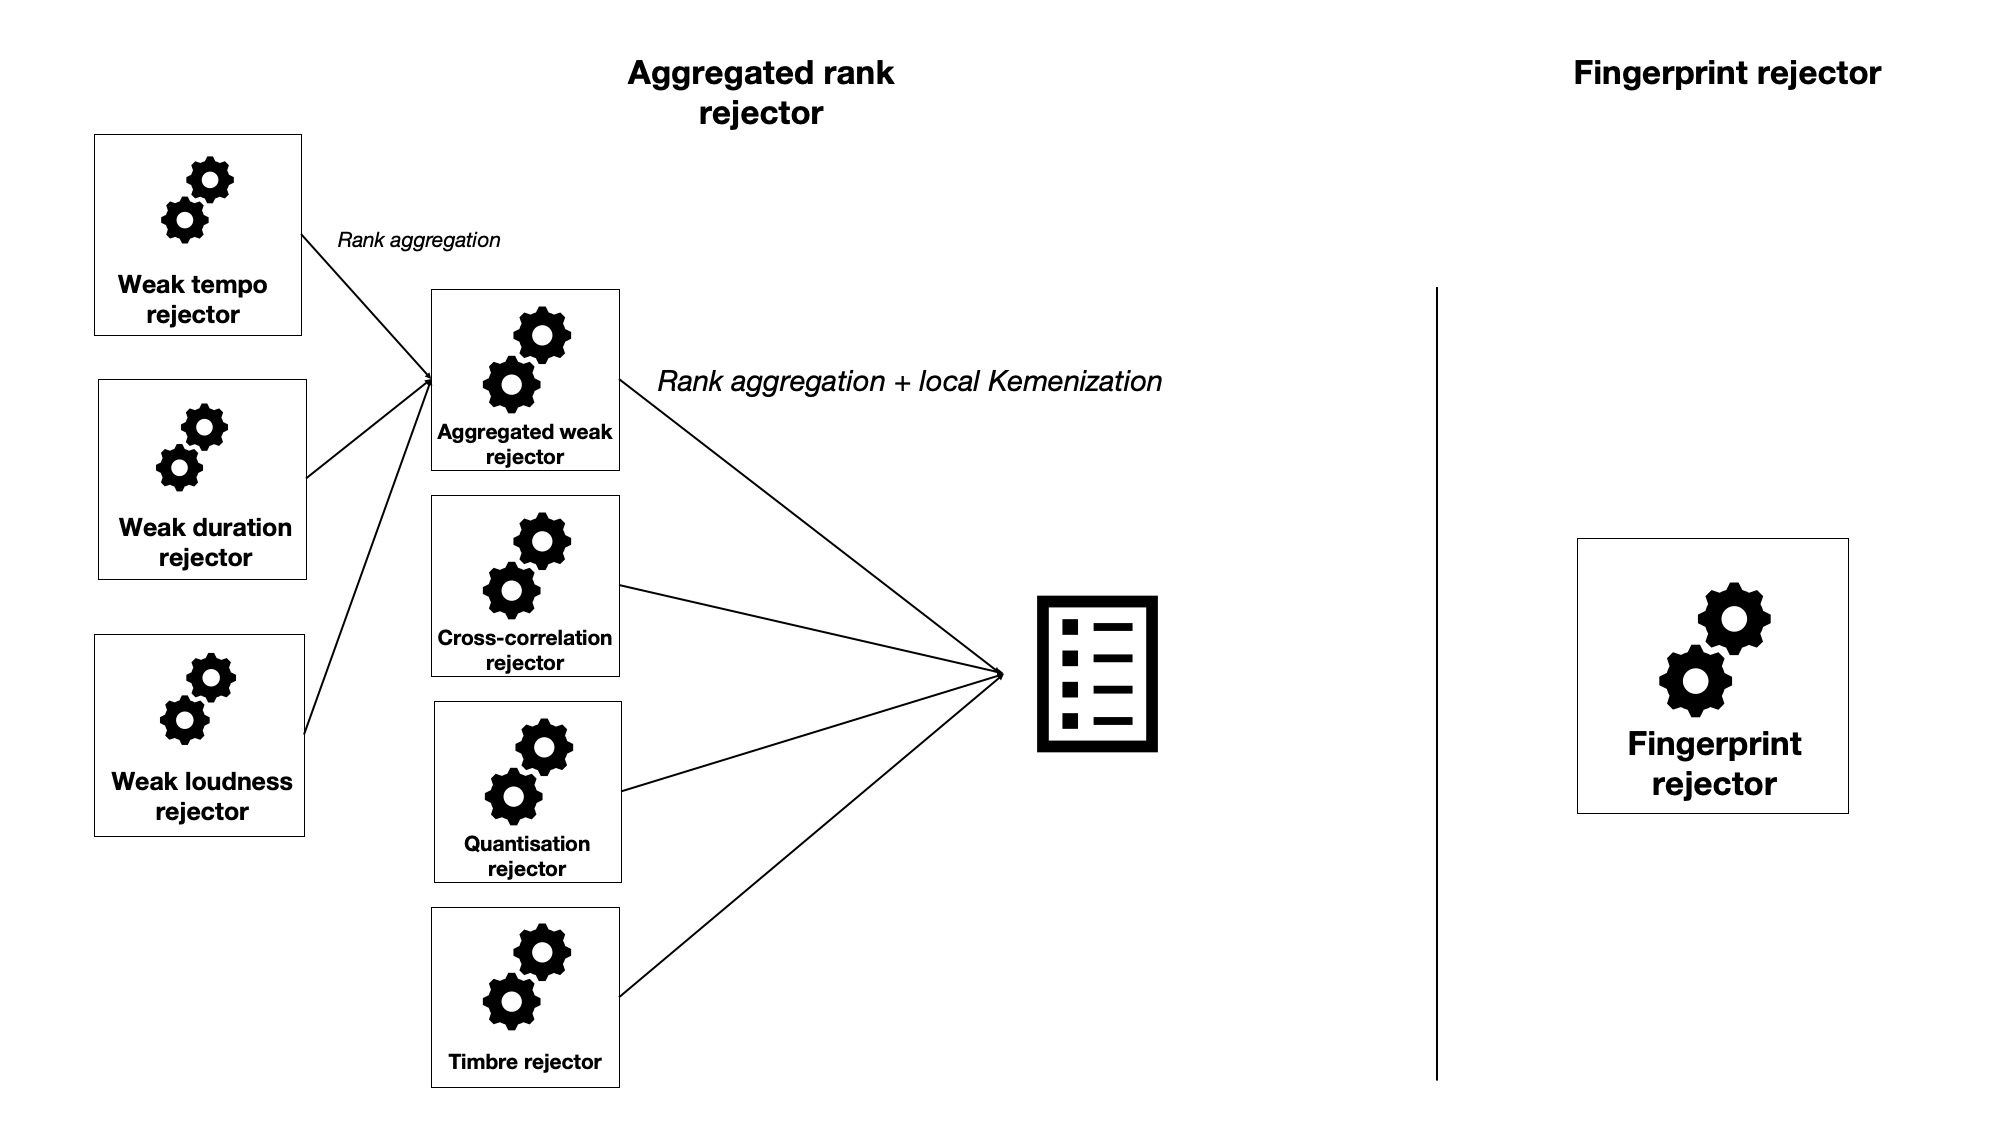
\includegraphics[width=\textwidth]{Algorithms/algorithm_diagram_3.jpg}
    \captionof{figure}[Algorithms diagram]{Diagram of chosen algorithms and the relationships between them. The aggregated rank rejector combines the results of 3 types of weak rejectors, as well as the quantisation, cross-correlation and timbre rejectors}
    \label{fig:algorithms}
\end{figure}

\section{Weak rejector} 
\label{sec:weakfeatures}

The weak rejector takes its name from the fact that it uses global single-valued
features of sound to calculate a similarity score. Weak features include tempo,
duration, loudness, average number of beats, etc. Those audio properties are
considered 'weak' since by themselves they cannot uniquely describe a song - the
majority of pop tracks from a certain era are composed with the same tempo, for
example \cite{slowpop}. As a consequence the results from weak rejectors are
inherently insignificant are usually not considered individually, but as
part of an aggregation with other results.

Each weak rejector takes a single audio feature as song representation. The
algorithm extracts the feature from each song in a dataset and from them it
creates a training set by combining each pair of songs in different ways. For
songs $A$ and $B$ with weak feature values of $f1$ and $f2$ respectively the
minimum ($min(f1, f2)$), maximum ($max(f1, f2)$), sum ($f1 + f2$), quotient
($\frac{f1}{f2}$) and absolute value of quotient of the difference divided by
the sum ($abs(\frac{f1 - f2}{f1 + f2})$) are taken. The generated data is used
as attributes to train an ExtraTrees classifier model. Extra randomised trees or
ExtraTrees classification is a form of random forest classification. In
contrast to the regular random forest implementation, ExtraTrees uses the whole
training data for each decision tree. Rather than calculating an optimal
cut-point, it also uses a random one. The direct benefits of using this
variation of random trees are higher computational efficiency while achieving
similar perfomance on average, in addition to better results on some specific
problems \cite{geurts2006extremely}.

The evaluation datasets used in this project are too small to generate an
ExtraTrees model which performs even adequate classification of songs. To gather
sufficient training data the weak features of 12,104 songs are extracted from
the music streaming service Spotify \cite{spotify}. The tracks are chosen based
on clique groupings from the SecondHandSongs (SHS) \cite{shs} dataset - the
largest dataset of covers songs aimed at academic research. While the full
dataset is difficult to obtain, information about the cliques structure within
it is easy to find. The extracted data is then combined into pairs using the
procedure outlined in the previous paragraph. A binary class is then assigned to
each pair entry depending on whether the pair of songs are covers or not.
Afterwards the training data is further split into a training set of 3773
cliques (8653 songs) and validation set containing 1573 cliques (3451 songs).
The metric used to validate the model performance is the area under the receiver
operating characteristic (ROC) curve - a curve resulting from the plot of the
true positive against the false positive rate of the validation results. ROC
analysis of such form is suitable as a validation metric for the selection of an
optimal model because it is independent of any potential cost function or cost
distribution \cite{wiki:roc}. Because we are solely working with weak feature
information the we can only validate based on correct and incorrect produced results.

After the training phase is complete each of the evaluation datasets is
converted into the training set format and passed to the model for class
prediction. The output result is a probability of every pair of songs being
covers. Grouping the results per song produces a database ordering that is
required by the evaluation task.

\section{Cross-correlation rejector} 
\label{sec:ccs}
The cross-correlation rejector uses chroma features as the main audio feature
describing each song. Chroma is another name for pitch class profiles, i.e. a
12-dimensional representation of the intensity distribution in each of the
twelve pitch classes part of the chromatic scale \cite{fujishima1999real}. Any
feature that at its core uses chroma to represent a song is a chroma feature.
That is why the terms harmonic pitch class profiles (HPCP) and chroma features
have a very similar definition, in fact HPCP is a type of chroma feature. The
main difference between chroma features is their method of extraction. Using
chroma features produces a chromagram - a pitch class versus time plot showing
the intensity of each pitch class at any time point (Figure
\ref{fig:chromagram}).

\begin{figure}[H]
    \centering
    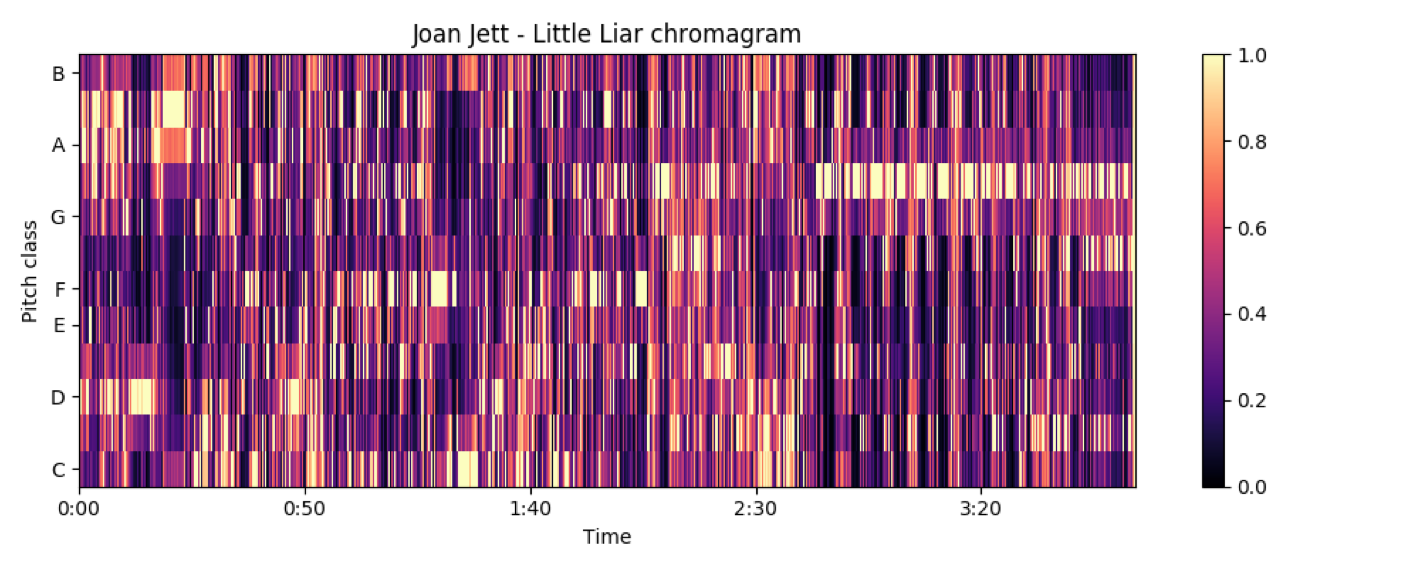
\includegraphics[width=\textwidth]{Algorithms/chromagram_picture.png}
    \captionof{figure}[Chromagram]{Chromagram of the song \textit{Little Liar} by Joan Jett}
    \label{fig:chromagram}
\end{figure}

The chroma features in the cross-correlation rejector are extracted by
performing short-time Fourier transform (STFT) analysis. It consists of running
Fourier transform on short segments of a signal to determine how the frequency
content changes over time \cite{gao2006non}. STFT improves upon the concepts of
regular Fourier transform by not only telling us what frequencies are contained
within the audio stream, but also at what time intervals does each frequency
appear.

The transformations are applied using the fast Fourier transform (FFT)
algorithm. The short segments are calculated over sliding overlapping windows as
illustrated on figure \ref{fig:stft}. The size of the sliding window is
determined by \textit{FFT window size} and the overlap between each window
depends on a parameter called \textit{hop length}. The actual window overlap is
calculated as the difference between the window size and the hop length.

\begin{figure}[H]
   \centering 
   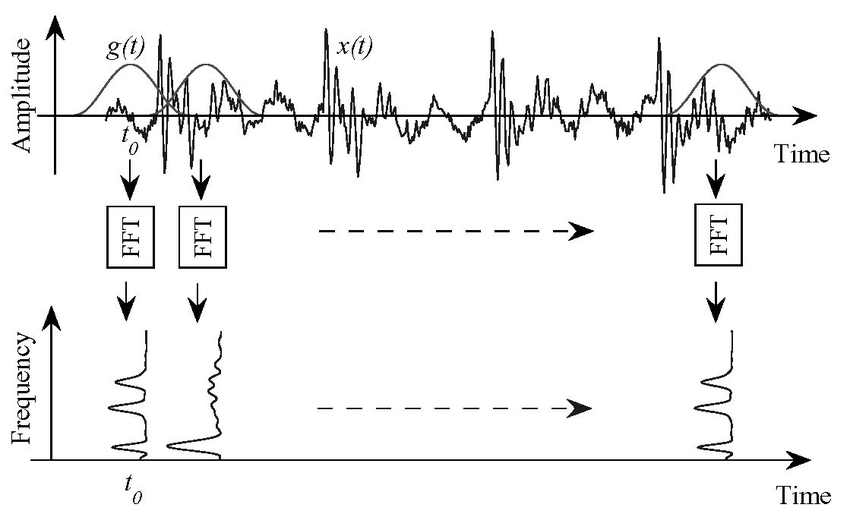
\includegraphics[width=\textwidth]{Algorithms/stft.png}
   \captionof{figure}[Short-time Fourier transform]{Workings of STFT on an audio signal $x(t)$. $g(t)$ is a function defined using the FFT window size and the hop length. The result of each FFT transformation is the amplitude and phase of frequency over the time period. \cite{gao2006non}}
   \label{fig:stft}
\end{figure}

The next step into obtaining chroma features for the cross-correlation rejector
is converting the spectrogram resulting from the STFT into a chromagram. Using
the standard mapping of pitch $A4 = 440 Hz$ and knowing that pitches in music
lay on an equal-tempered scale we can calculate the remaining pitches (relative
to A4) from the frequency spectrum.  We then aggregate all pitches belonging to
the same pitch class and that gives us the chroma value of the chroma value
corresponding to the class.

The conversion from frequency to pitch is regulated using a specification
defining a function to be used when the pitches relative to $A4$ are calculated.
This standardisation is commonly referred to as \textit{tuning standard}. The
paper describing the cross-correlation rejector does not specify what tuning was
used to generate the chroma features, so a library implementation of chroma
feature extraction was used in the benchmark. To further explain the conversion
of frequency to chroma an example using the \textit{MIDI tuning standard} is
presented. Figure \ref{fig:spectrotochroma} follows each stage of the procedure.

The MIDI tuning covers a range of 128 frequencies enumerated from 0 to 127. A4
(which again corresponds to $440 Hz$) is assigned number 69 and all other
pitches are calculated using the equation:

\begin{figure}[H]
    \label{fig:midiequation}
    \begin{equation}
       d = 69 + 12 \log_{2}(\frac{f}{440 Hz})
    \end{equation} 
    \captionof{figure}[MIDI Tuning pitch calculation equation]{Calculating pitch from frequency $f$ based on MIDI tuning standard \cite{mts}.}
\end{figure} 

This gives us a song representation similar to the one from
\ref{fig:spectrotochroma} c). The final step is to sum all MIDI pitch
coefficients into their corresponding pitch classes and obtain the chromagram
from \ref{fig:spectrotochroma} d).

\begin{figure}[H]
    \centering
    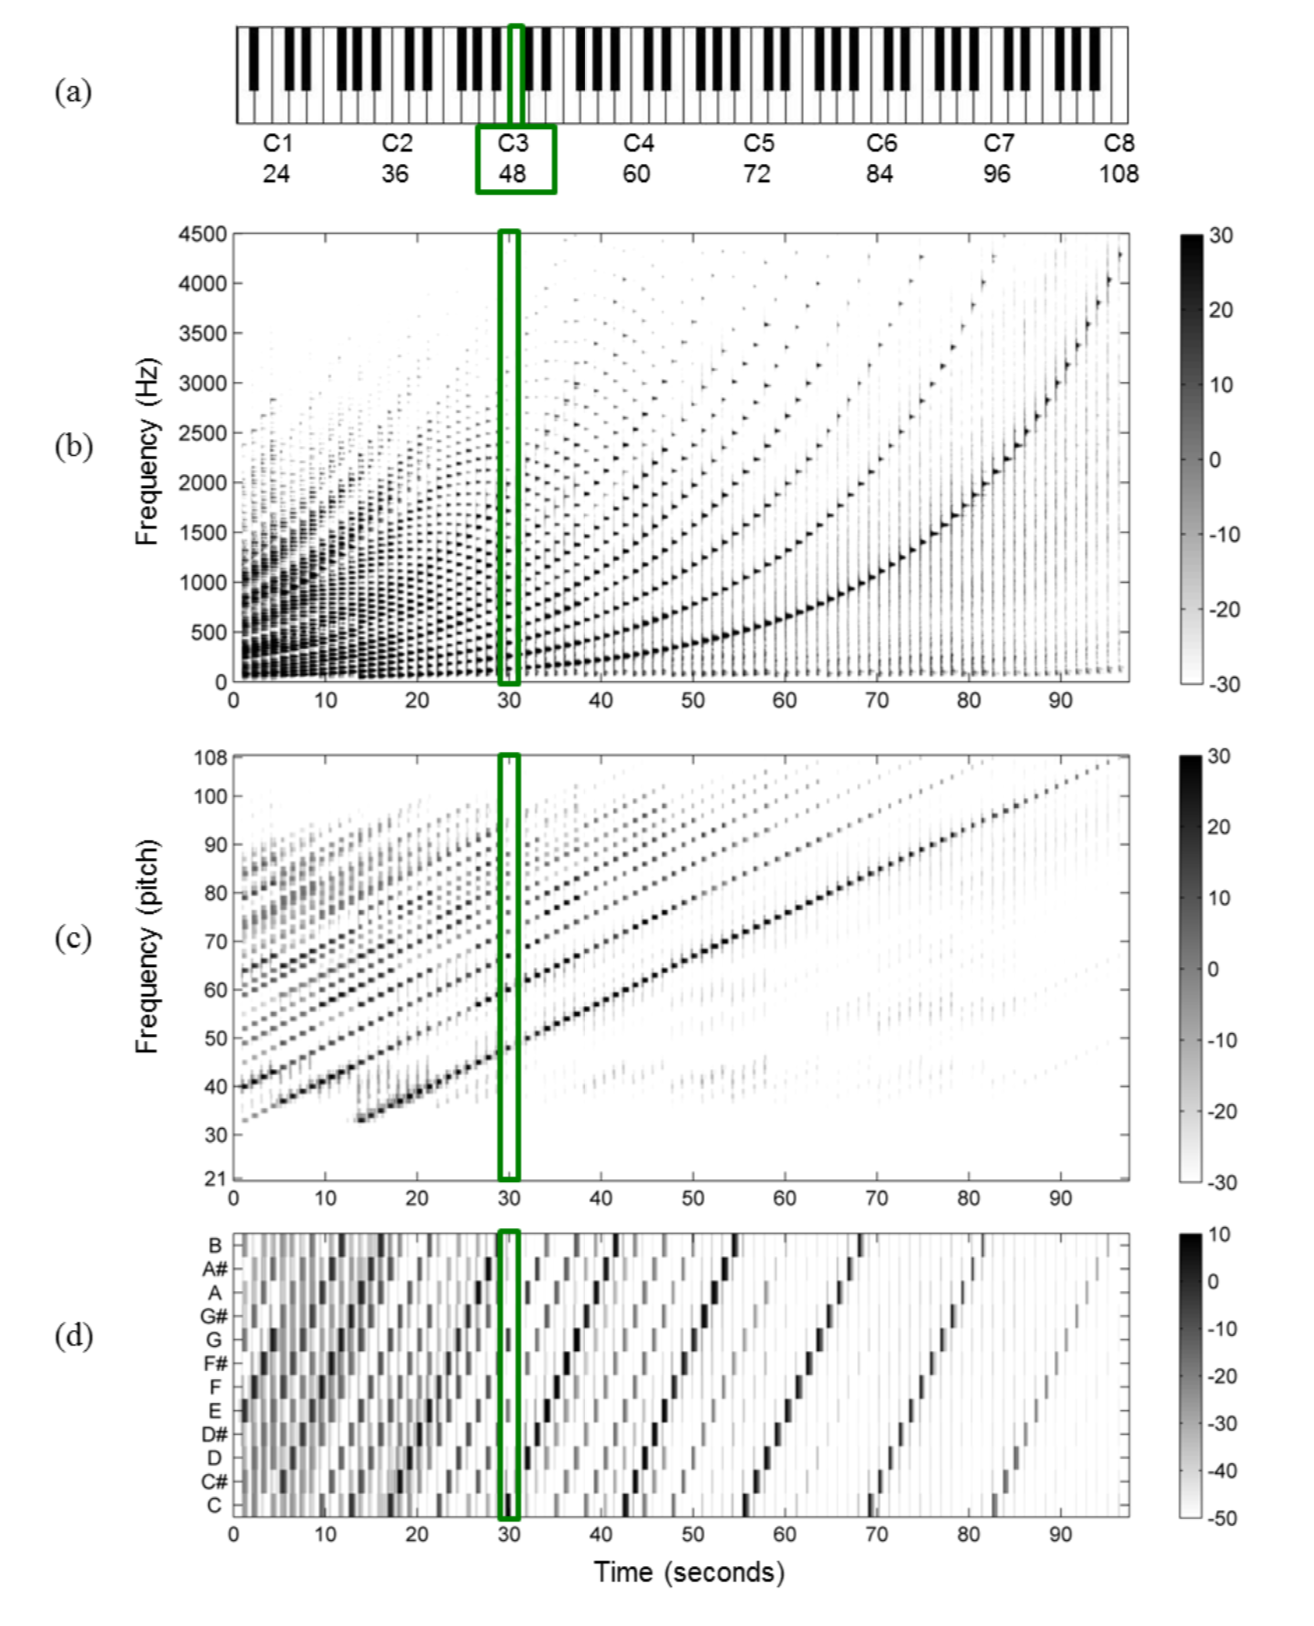
\includegraphics[width=0.69\textwidth]{Algorithms/spectrogram_to_chromagram.png}
    \captionof{figure}[Spectrogram to chromagram conversion]{The separate stages of a spectrogram to chromagram conversion of a piano recording of the chromatic scale from A0 to C8 using MIDI tuning. \cite{mullershort}. a) The equal-tempered scale represented by the keys of a piano, with the pitch C3 mapped to 48 according to MIDI Tuning b) A spectrogram of the song, with the time frame where C3 was played marked in red c) Pitch log-frequency representation of the spectrogram d) Resulting chromagram}
    \label{fig:spectrotochroma}
\end{figure}

\paragraph{}
The chroma features in the cross-correlation rejector are
\textit{beat-synchronous}. This means that the period over which a chroma
feature is obtained is every beat of the song, rather than a shorter time
segment. The technique is very popular within cover song algorithms due to its
ability to make comparisons between songs invariant to tempo, a property which
is often modified by the cover song artists. Understanding beat detection in
detail was beyond my abilities and a library implementation of a beat tracker
created by the algorithm creators is directly used to obtain a result
\cite{librosa_beat}.

\paragraph{}
The resulting chromagrams for two songs are then scaled to unit length, so that
the sum of all dimensions of the chroma vector has a sum of 1. The
representation of the longer song is also shortened to be equal to the one of
the shorter song. The chromagram matrices are then cross-correlated. To account
for variations in the structure or pitch of the cover songs the shifts of the
chromagrams between -500\dots500 beats are considered. The resulting intervals
of peak values of peaks in the resulting cross-correlation matrix indicate a
strong match between both tracks. Figure \ref{fig:cross-correlation} shows the
correlation process of two chromagrams. The blue line in the cross-correlation
matrix indicates the strong similarity detected.

The similarity score that the rejector returns is the reciprocal value of the
highest peak value in the cross correlation matrix.

\begin{figure}
    \centering
    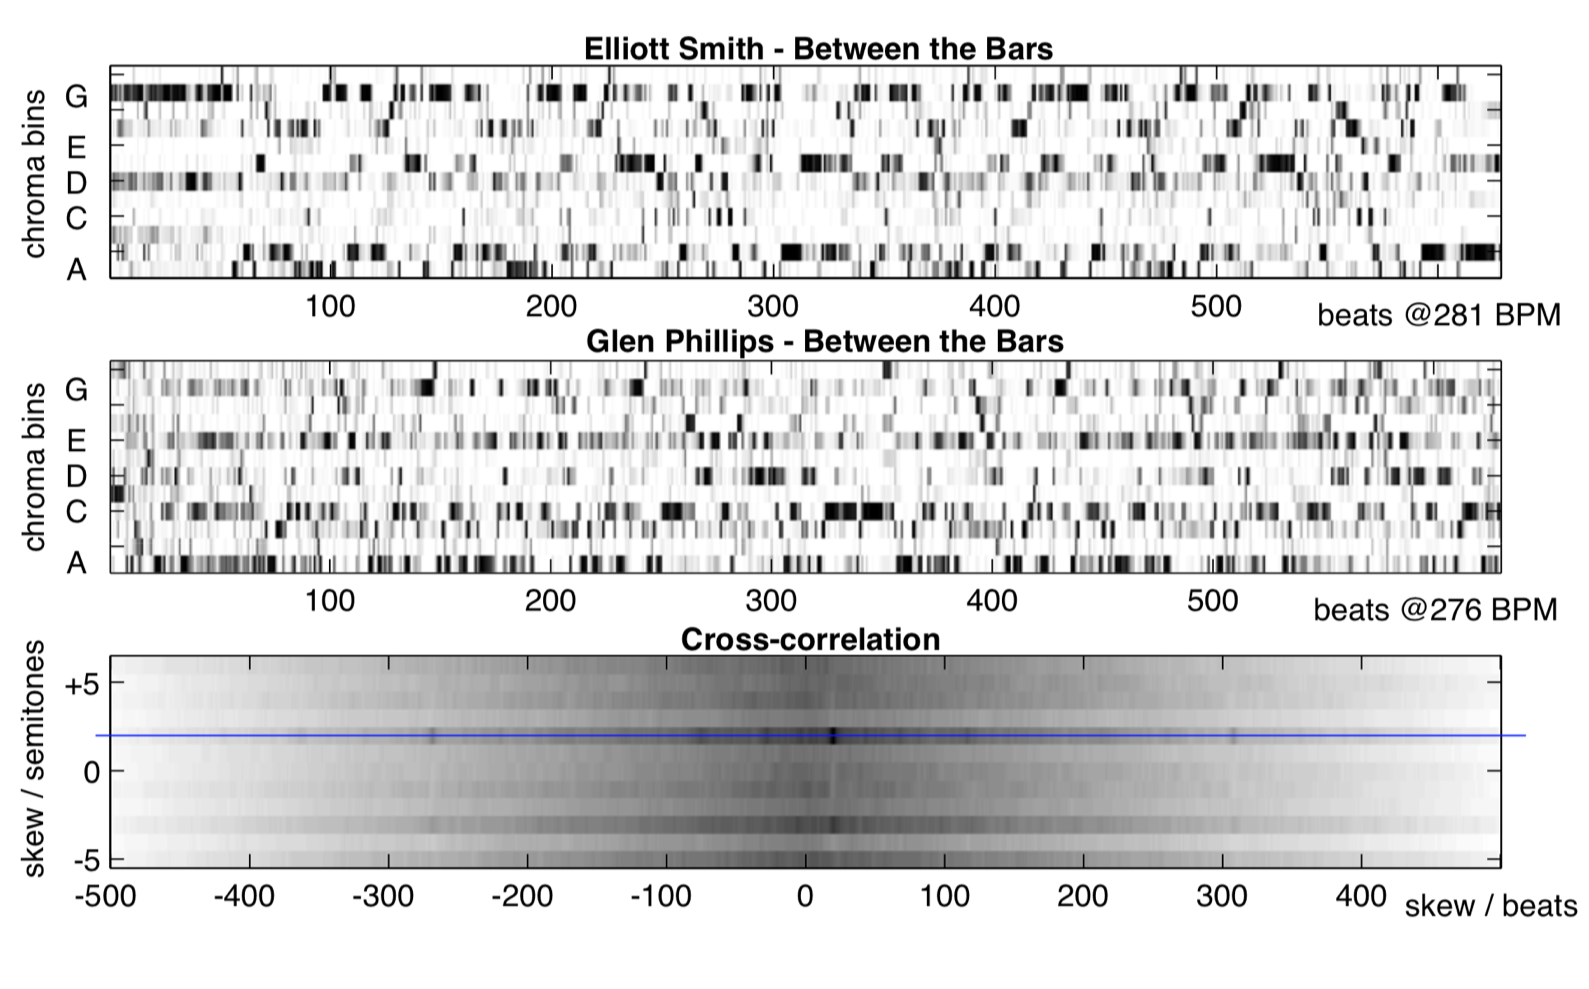
\includegraphics[width=\textwidth]{Algorithms/cross-correlation.png}
    \captionof{figure}[Cross-correlation of chromagrams]{Extracted chromagrams of two cover songs and the resulting cross-correlation \cite{ellis2007identifyingcover}}
    \label{fig:cross-correlation}
\end{figure}

\section{Quantisation rejector}
\label{sec:quantisation}

The dominant audio feature in the quantisation rejector is again chroma vectors
which are beat-synchronous and unit normalised. The extraction implementation is
the same, with some modifications to the FFT window size and hop length
parameters. The general idea of the rejector is to represent songs using
\textit{codewords} which are generated using K-means clustering of a large
number of chroma vectors. The resulting cluster centers are the codewords. Each
song is then represented using a histogram showing the codewords frequency for
each track. As illustrated in figure \ref{fig:quantisation} the approach leads
to visible similarity between cover songs. 

\begin{figure}[H]
    \centering
    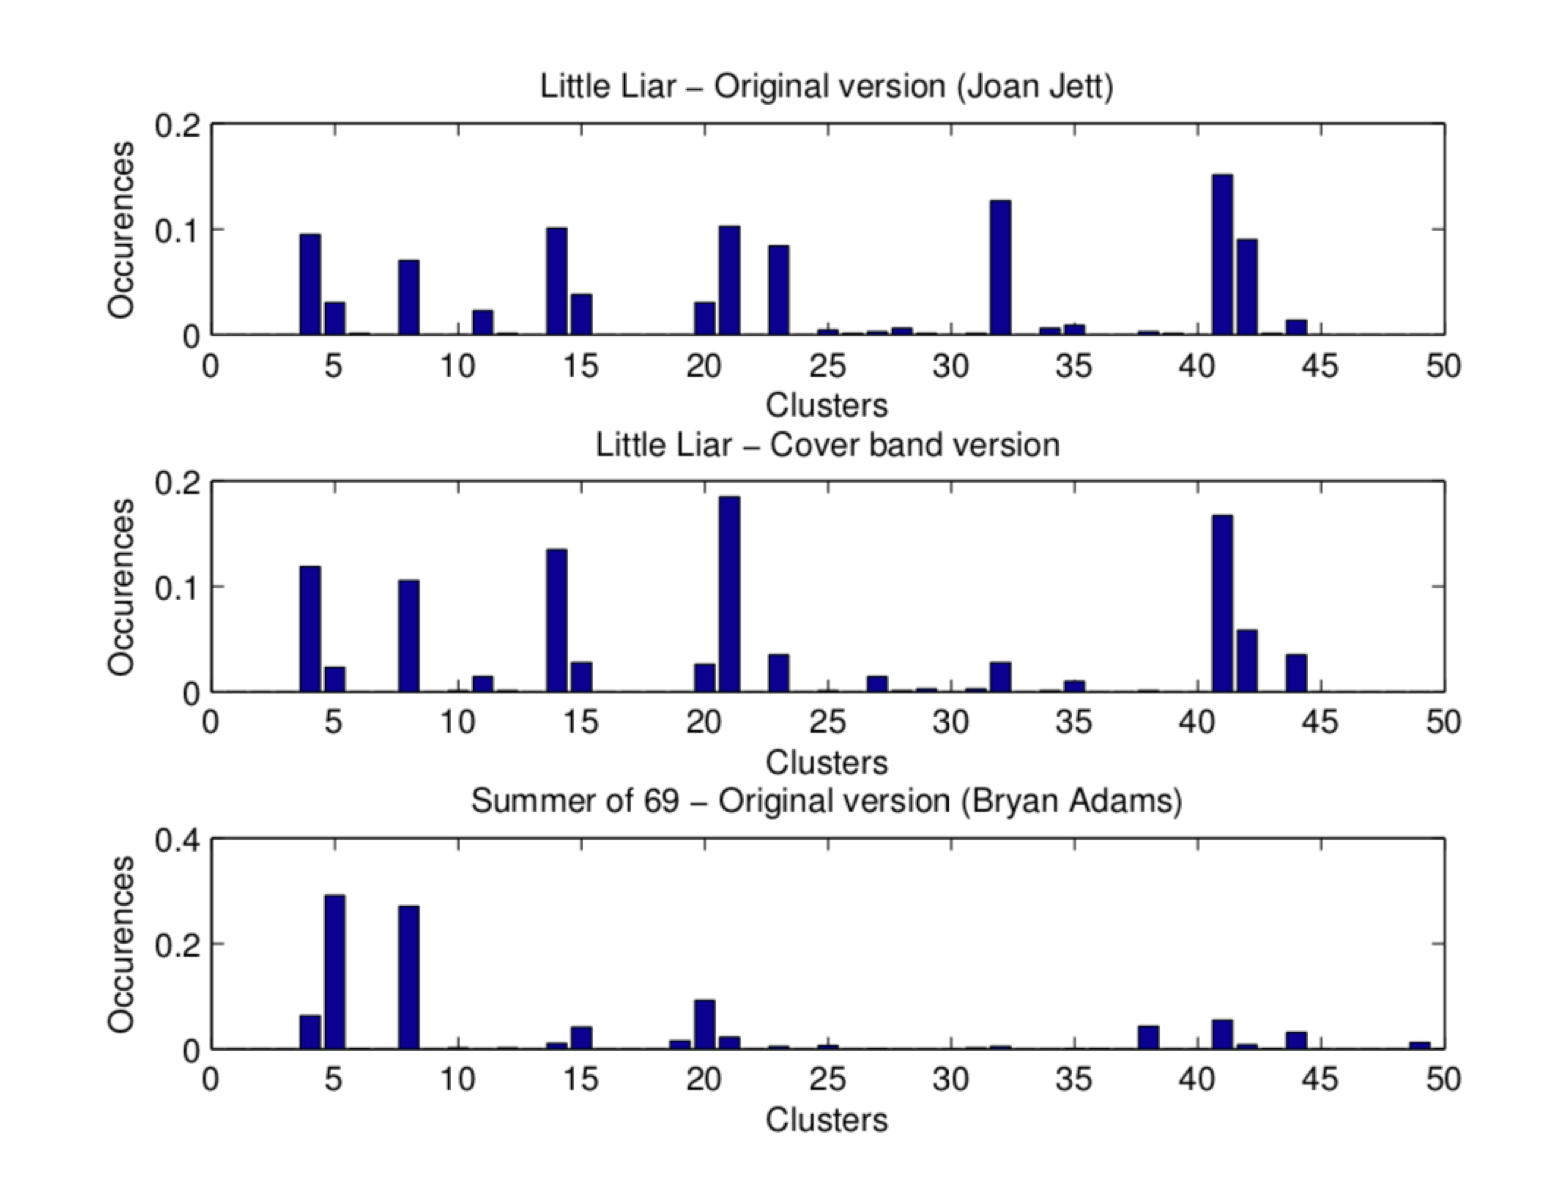
\includegraphics[width=\textwidth]{Algorithms/quantisation.png}
    \captionof{figure}[Quantisation example]{Histogram representations of songs utilising codewords. The first two histograms illustrate the visual similarity occurring between two cover, in comparison to the third song which is not related to the first two \cite{osmalskyj2013efficient}}
    \label{fig:quantisation}
\end{figure}

Sometimes a cover song can shift up or down the overall pitches of the original
by a fixed interval. This technique is called \textit{key transpositions}. To
take possible transpositions into consideration the quantisation rejector
implements \textit{Optimal Transposition Index (OTI)} \cite{serra2008audio}. It
is a calculation on the number of positions one of the histograms needs to be
shifted in order to achieve best possible alignment with the other. For two
histograms represented as $n$-dimensional vectors $\vec{A}$ and $\vec{B}$, where
$n$ is the number of codewords used, the OTI is derived from:

\begin{figure}[H]
   \begin{equation}
       OTI(\vec{A}, \vec{B}) = \argmax_{0 \leq m \leq {n-1}}\{\vec{A} \cdot circshift_{R}(\vec{B}, m)\}
   \end{equation}
   \captionof{figure}[Optimal Transposition Index (OTI) equation]{OTI equation}
\end{figure}

$circshift_R$ is a function shifting the vector $\vec{B}$ $m$ positions to the
right. The shift is circular, which means that the last element of the vector
becomes the first one after every position shift. The operator $\cdot$ specify a
dot product operation between both vectors. The OTI is used to shift one of the
vectors to achieve best alignment between both songs:
\begin{figure}[H]
\begin{equation}
    \vec{A^{Tr}} = circshift_R(\vec{A}, OTI(\vec{A}, \vec{B})) 
\end{equation}
\captionof{figure}[Transposing a histogram based on OTI]{Shifting $\vec{A}$ to best align with $\vec{B}$}
\end{figure}

The performance of each K-means clustering model during training is evaluated
through the sum of squared distances of each clustered point to their closest
cluster center, a metric called \textit{inertia} \cite{scikit-learn}. A low
inertia indicates a a good separation of the points and therefore a good model.

The final similarity metric returned
by the quantisation rejector is the cosine similarity between both histograms.

\section{Timbre rejector} 
\label{sec:timbre}
Beat synchronisation deals with tempo variations, but cannot handle any key
changes in a cover song compared to the original. Chroma features also mix all
octaves into pitch classes which obscures the nuances in the "colour" of sound.
The timbre rejector aims to present a solution by examining the relative change
of timbre over time.

The timbre rejector uses \textit{Mel-frequency cepstrum coefficients (MFCCs)} as
audio features due to their ability to preserve the timbral information after
transformation of the signal \cite{tralie2015cover}. MFCCs take the cepstrum of
a song and project it on a mel scale. The main purpose of the feature is to
serve as a bridge between the ways humans perceive sound (logarithmic frequency
distinction, mel scale, etc) with the mechanics of musical instruments, in
particular harmonics generation.

\textit{Cepstrum} was originally created to describe a technique for detecting
echoed signals in measured time series \cite{martin1986power}. Since then it has
been applied in many speech recognition problems \cite{muda2010voice}
\cite{viikki1998cepstral}, and now it is also used in other MIR tasks such as
cover song identification.

Cepstrum is informally defined as a nonlinear "spectrum of a spectrum". All
types of cepstrum are usually obtained through a configuration of Fourier
transform of a Fourier transform. For MFCCs we need to obtain the \textit{power
cepstrum} $c[n]$ defined as:
\begin{figure}[H]
    \begin{equation}
        c[n] = |\mathcal{F}^{-1}\{\log{}(|\mathcal{F}\{ x[n]\}|^2)\}|^2
    \end{equation}
    \captionof{figure}[Power cepstrum equation]{Derivation of a power cepstrum, where $\mathcal{F}$ denotes a discrete Fourier transform (DFT), $\mathcal{F}^{-1}$ is the inverse discrete Fourier transform (IDFT) and $x[n]$ is the audio signal to be transformed \cite{wiki:cepstrum}}
\end{figure}

\paragraph{}
Another representation of the operation is available on figure \ref{fig:powerspectrumsequence}.

\begin{figure}[H]
    \centering
    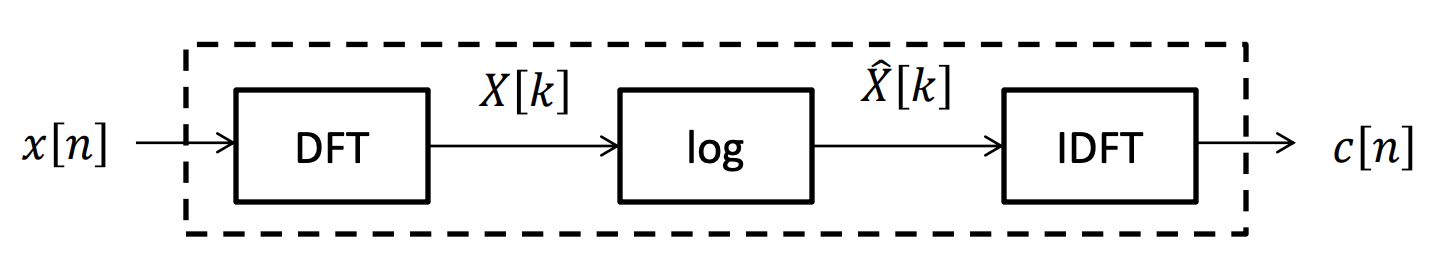
\includegraphics[width=\textwidth]{Algorithms/powercepstrum.png}
    \captionof{figure}[Sequence diagram of obtaining power cepstrum]{Sequence of Fourier transforms to obtain power spectrogram \cite{cepstrumgraph}}
    \label{fig:powerspectrumsequence}
\end{figure}

By applying DFT we obtain the power spectrum of a song - a projection of sound
power versus frequency resulting in a log spectrogram such as the one from
figure \ref{fig:powercepstrum}. The aim of the power cepstrum is to measure the
periods of the resulting functions - on figure \ref{fig:powercepstrum} the
frequency with a longer period (described by the dashed line) is a
representation of the fundamental frequency, while the one with lower period
represents the harmonic overtones. By applying IDFT to the spectrogram we derive
the power cepstrum in the second graph of figure \ref{fig:powercepstrum}. The
peak in the the cepstrum represents the fundamental frequency and its period as
at \textit{quefrency} T. A quefrency is intended to denote the inverse of
frequency as a time domain unit \cite{cepstralanalysis}. On the left side of the
quefrency axis we have peaks which represent the periods of each harmonic.

By having the period sizes of the harmonics relative to each other we can
gain information about the harmonic evolution over time. This harmonic
information tends to be present even in cover songs significantly different than
the original \cite{tralie2015cover}.

MFCCs are coefficients that are part of the \textit{Mel-frequency
cepstrum}, a variation of the power cepstrum where the extracted peaks of
each harmonic are projected on a mel scale based on their frequencies. They are
extracted as 20-dimensional vectors from a song.

\begin{figure}[H]
    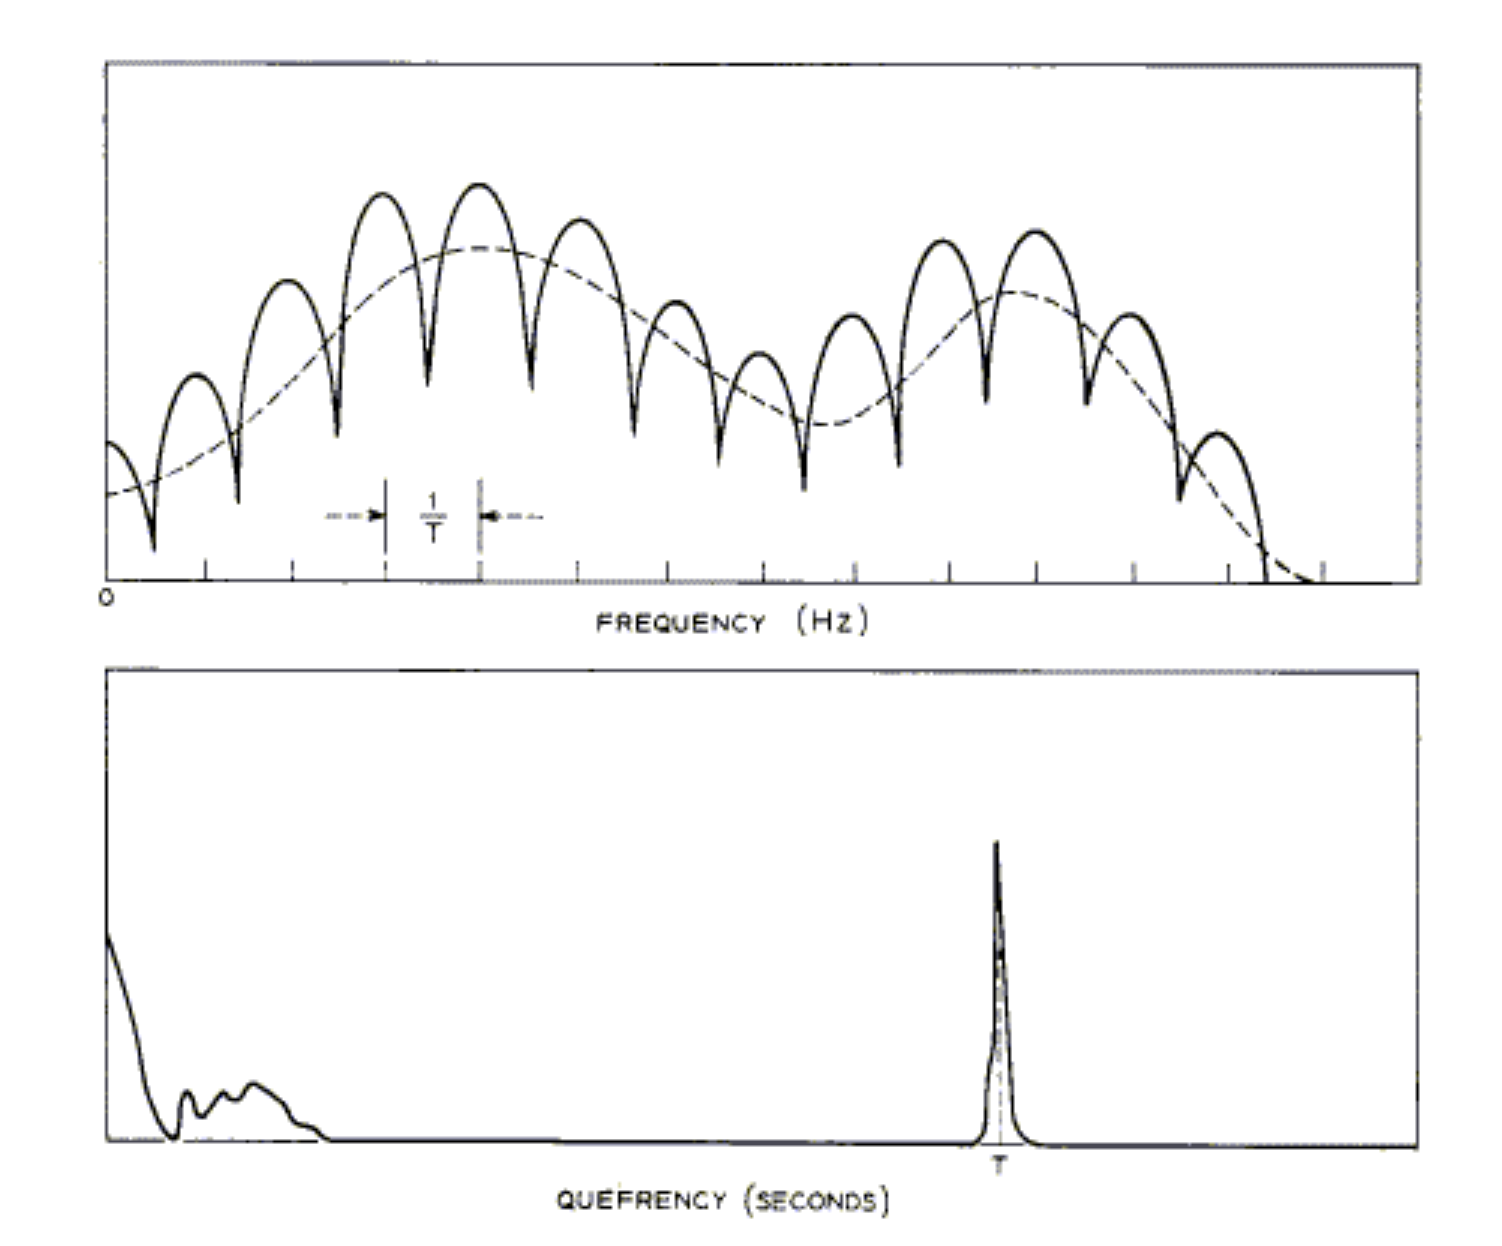
\includegraphics[width=\textwidth]{Algorithms/powercepstrum2.png}
    \captionof{figure}[Comparison between a log spectrogram and a power cepstrum]{Spectrogram after applying DFT on the signal and  a power cepstrum of it. $F(W)$ is equivalent to $\mathcal{F}\{x[n]\}$ \cite{noll1967cepstrum}}
    \label{fig:powercepstrum}
\end{figure}

Just like most of the previous rejectors, MFCCs in the timbre rejector are
extracted using over the identified beat intervals in a track. There is one
significant difference however - each extraction time frame is a \textit{block}
enclosing $B$ time-contiguous beat intervals. Every two successive blocks
overlap in a way that only the first beat of the first block and the last beat
of the second block differ between two blocks. For a song which contains $N$
beat intervals, the total number of blocks is $N - B + 1$. The MFCC features are
extracted from each block using \textit{discrete Cosine transform (DCT)}, a
Fourier transform very similar to the discrete Fourier transform. As with STFT,
DCT requires a sliding window size and hop length. The specific parameters for
the MFCC extraction are discussed in chapter \ref{chap:benchmark}. One MFCC
vector is extracted over every sliding window.

The group of 20-dimensional MFCC vectors within one block is called a
\textit{20-dimensional point cloud}. A self-similarity matrix (SSM) is
constructed from every point cloud. If we have a cloud $X \in \mathbb{R}^{M
\times 20}$ where $M$ is the number of points in the cloud, the derived SSM
matrix $D$ has dimensions $M \times M$. As a pre-processing method aiming to
normalise for loudness we center the cloud on its mean and scale each point to
unit norm:
\begin{equation}
    \overset{\wedge}{X} = \{\frac{x - mean(x)}{||x - mean(x)||_2}:\; x \in X\}
\end{equation}

Where the distance metric is \textit{L2 vector norm}, defined as $||x||_2 =
\sqrt{\sum_ix_i^2}$. Each element of the SSM is then calculated using:
    \begin{equation}
        D_{ij} = |\overset{\wedge}{X}[i] - \overset{\wedge}{X}[j]||_2
    \end{equation}

The length of a beat segment depends strictly of the tempo of a track, therefore
it is common that we end up with different SSM dimensions for each song. To
enable comparisons between matrices from different songs, all SSMs are resized
to a dimension $d \times d$, where $d$ is an empirically selected parameter.

\begin{figure}[H]
    \centering
    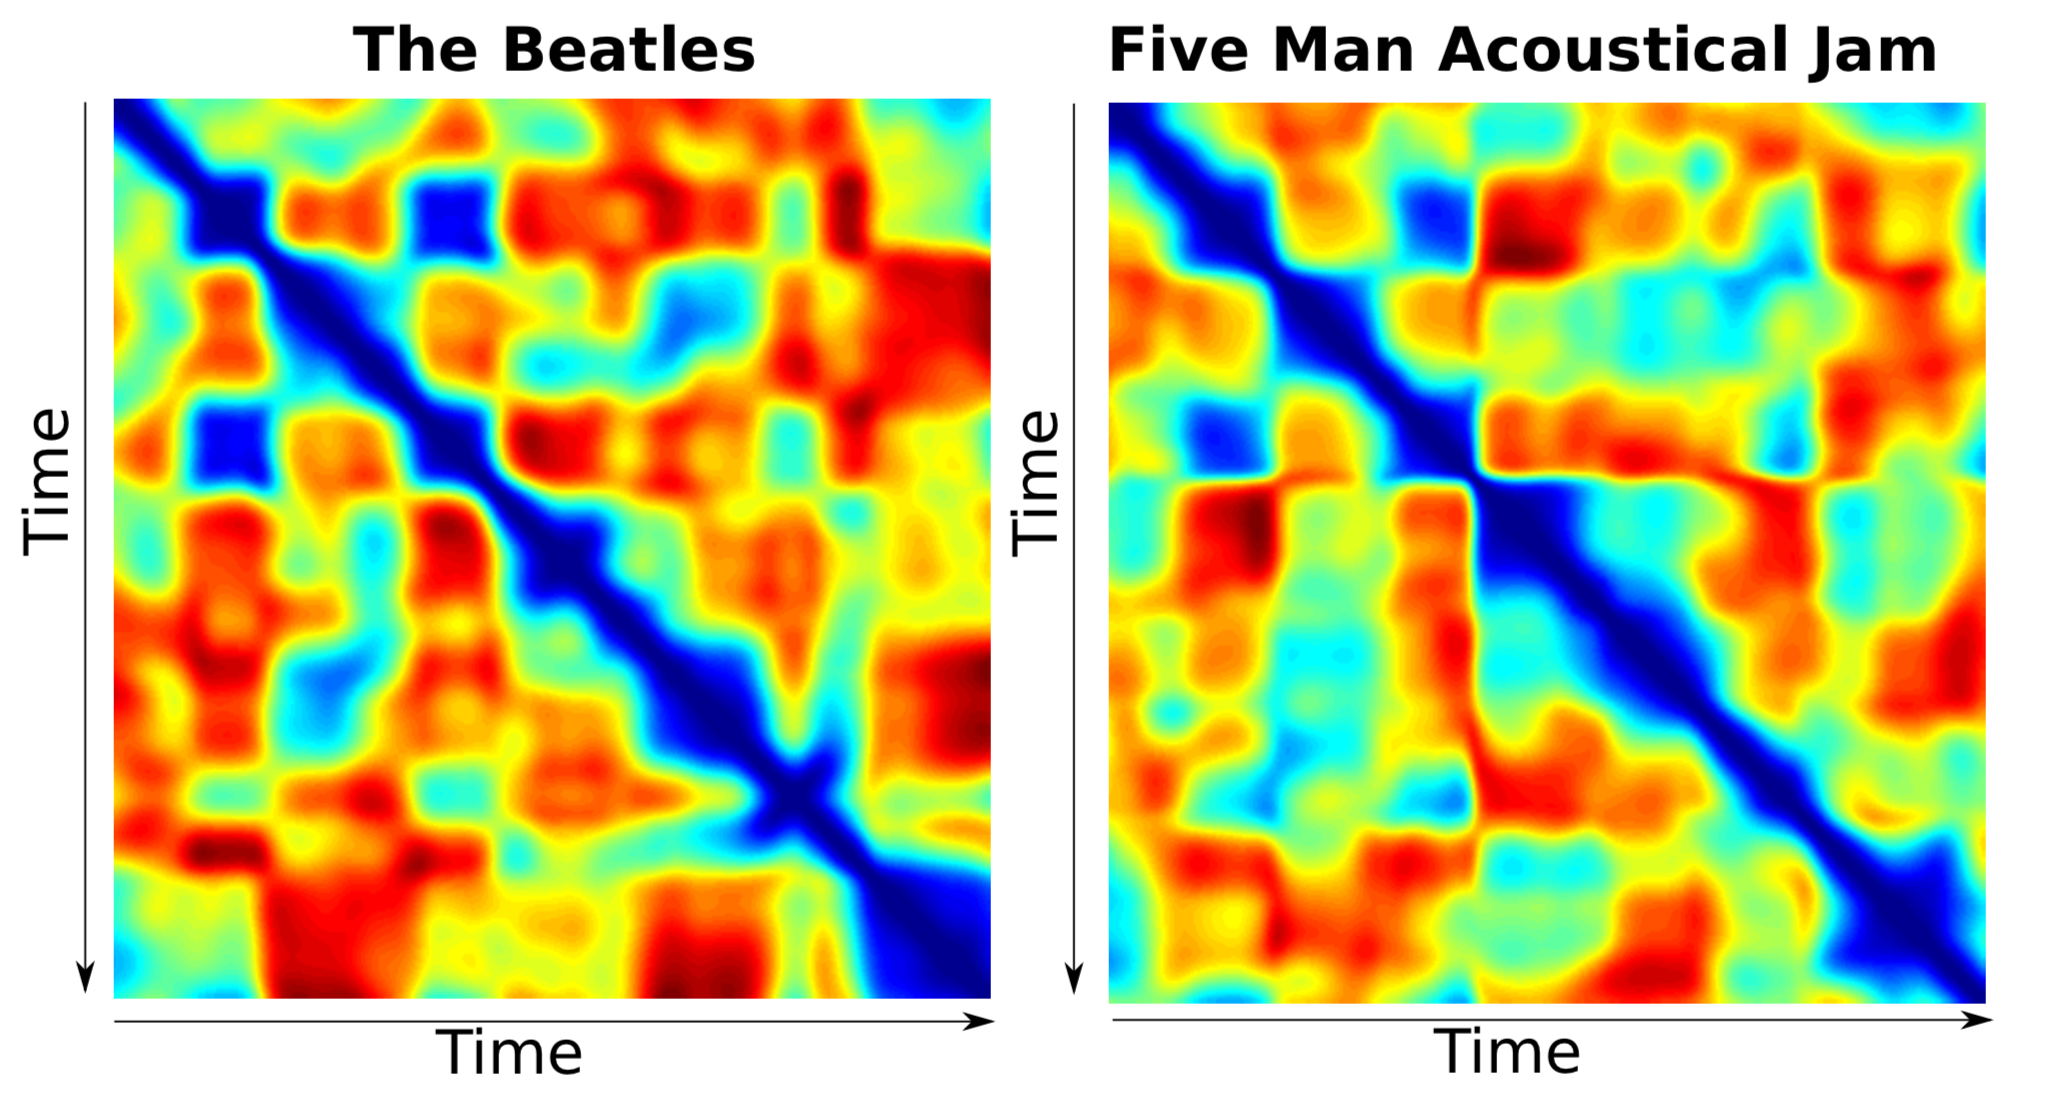
\includegraphics[width=0.6\textwidth]{Algorithms/ssms.png}
    \captionof{figure}[Self-similarity matrices from MFCCs]{Example self-similarity matrices across 4 beats of the song "We Can Work It Out" by The Beatles (left) and its cover version created by Five Man Acoustical Jam (right). Some similarity is clearly visible \cite{tralie2015cover}}
    \label{fig:ssmexamples}
\end{figure}

The final song representation is a set of all SSMs extracted from a
song and ordered by blocks. The matrices for each database song is generated and
stored, as it is needed for comparisons with the query song.

\paragraph{}
When a query song is passed to the timbre rejector, the algorithm extracts the
MFCCs and constructs the SSM representation of a song as described above. The
query song is then paired with every database song and a cross-similarity matrix
(CSM) is created for each pair. By having a set of $N$ SSMs for song A and a set
of $M$ SSMs for song B, the CSM has dimensions $N \times M$, with an element
calculated using:
\begin{equation}
    CSM_{ij} = ||SSMA_i - SSMB_j||_2
\end{equation}

$SSMA_i$ and $SSMB_j$ identify the $i^{th}$ block from song A and the $j^{th}$
block from song B respectively. The distance metric is the \textit{Frobenius
norm}, where given a matrix $X$ of size $D \times E$:
\begin{equation}
    ||X||_2 = \sqrt{\sum_{i=1}^D\sum_{j=1}^E|a_{i, j}|^2} : \; a \in X
\end{equation}

To obtain a similarity score, we need to binarise the CSM. The binary matrix is
computed using mutual fraction $\kappa$ nearest neighbours, i.e. $B^M_{ij} = 1$
if $CSM_{ij}$ is within the $\kappa M^{th}$ smallest values in row $i$ and also
within the $\kappa N^{th}$ smallest values in column $j$ of the CSM
\cite{tralie2015cover}. The value of $\kappa$ is a proportion between 0 and 1.

\begin{figure}[H]
    \centering
    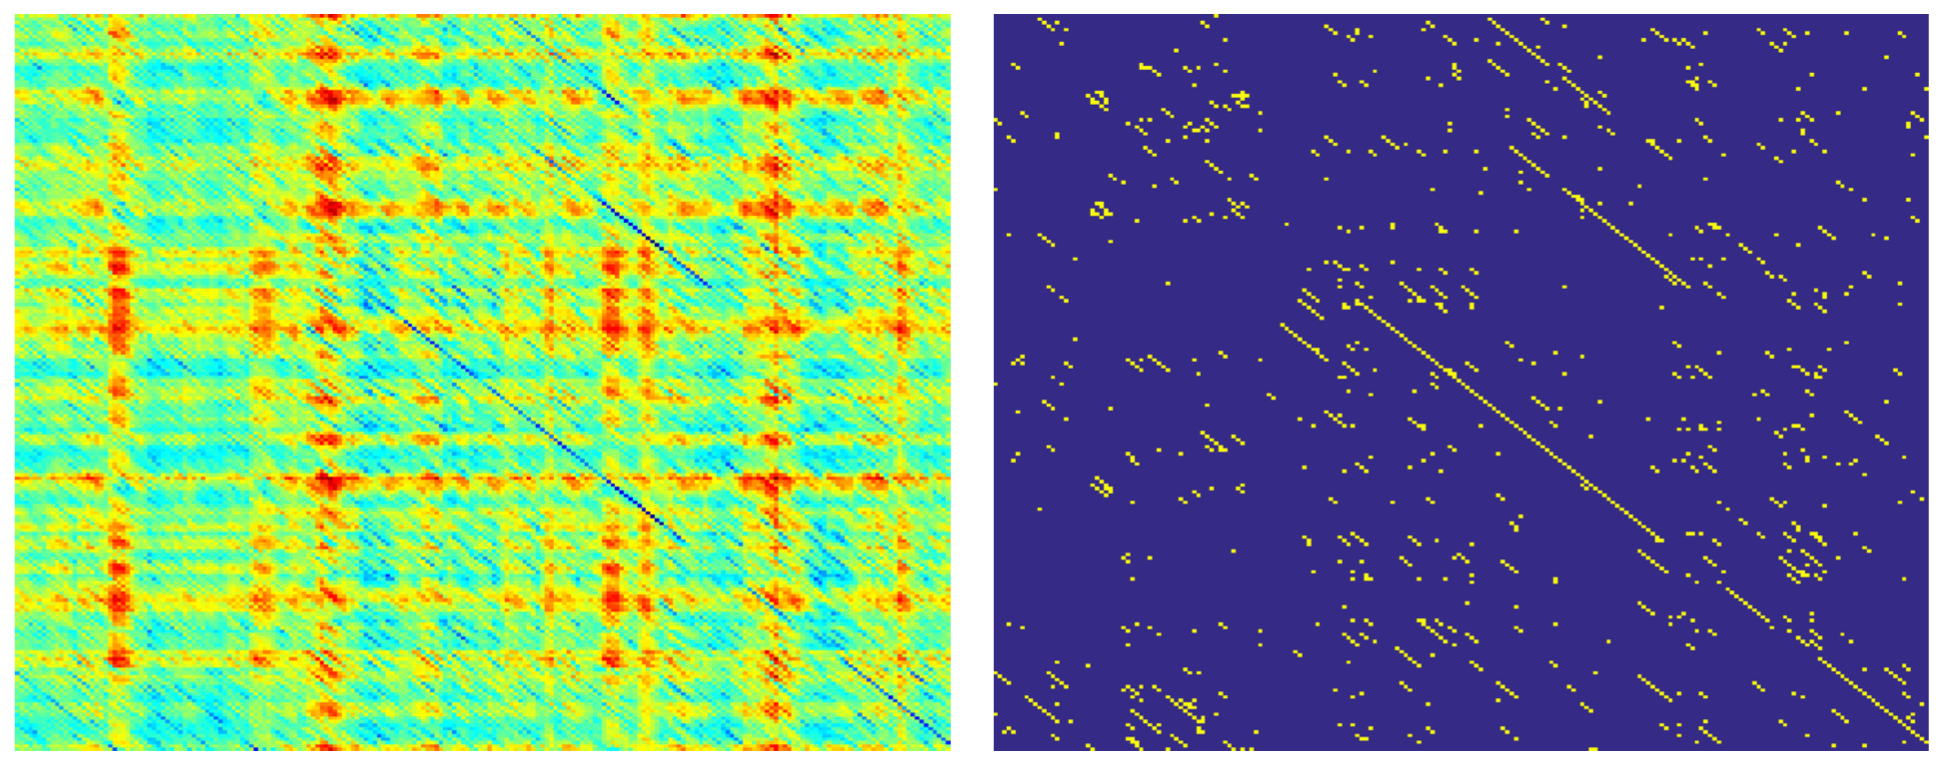
\includegraphics[width=0.6\textwidth]{Algorithms/csmbm.png}
    \captionof{figure}[Cross-similarity matrix and binary matrix from two cover songs]{Cross-similarity matrix (left) which is then converted to a binary matrix (right). The two songs examined are two versions of "We Can Work It Out" by The Beatles and Five Man Acoustic Jam \cite{tralie2015cover}}
    \label{fig:csmbm}
\end{figure}

The final step of the rejector is to measure similarity using
\textit{Smith-Waterman (SW) algorithm}. It presents a technique for detecting
the best local alignment between tracks by evaluating the binary matrix from the
previous step. The rejector implementation prefers local over global alignment
due to the fact that cover versions of songs could add custom intro, outro and
bridge sections, but be very similar otherwise to the original. Smith Waterman
creates another matrix $D$ from the binary matrix based on the following
recursive function:
\begin{equation}
   D_{ij} = max \begin{cases}
    D_{i-1, j-1} + (2\delta(B^M_{i-1, j-1}, 1) - 1) + \Delta(B^M_{i-2, j-2}, B^M_{i-1, j-1}), \\
    D_{i-2, j-1} + (2\delta(B^M_{i-1, j-1}, 1) - 1) + \Delta(B^M_{i-3, j-2}, B^M_{i-1, j-1}), \\
    D_{i-1, j-2} + (2\delta(B^M_{i-1, j-1}, 1) - 1) + \Delta(B^M_{i-2, j-3}, B^M_{i-1, j-1}), \\
    0
   \end{cases}
   \label{eq:sw}
\end{equation}

The sign $\delta$ represents Kronecker delta function, which given two variables
$i$ and $j$ it returns values:
\begin{equation}
    \delta_{ij} = \begin{cases}
       0\; if \; i \neq j, \\
       1\; if \; i = j
    \end{cases}
\end{equation}

Based on the Kronecker delta the term $2\delta(B^M_{i-1, j-1}, 1) - 1$ assigns
score of +1 if there is a match between the two songs, and -1 if there is
mismatch between both tracks.

The $\Delta$ function is called \textit{affine gap penalty} and assigns a score
to an identified gap. The scoring takes the form of:
\begin{equation}
    \Delta(a, b) = \begin{cases}
        \;\;\:0\; if \; b = 1, \\
       -0.5\; if \; b = 0, a = 1, \\
       -0.7\; if \; b = 0, a = 0 
    \end{cases}
\end{equation}

The Smith-Waterman algorithm configuration is adapted to prioritise diagonal
alignment, rather than horizontal or vertical one. Any gaps that occur on the
diagonal are appearing in both songs almost simultaneously in time, which is
also a form of similarity. At the same time if large gaps happen in a horizontal
or vertical line, they would indicate a large mismatch between both songs.

An illustration of the different matrix evaluated is given in figure
\ref{fig:swworkings}. The resulting SW matrix for the two versions of "We Can
Work It Out" is shown on figure \ref{fig:swmatrix}.
\begin{figure}[H]
    \centering
    \begin{minipage}{.5\textwidth}
      \centering
      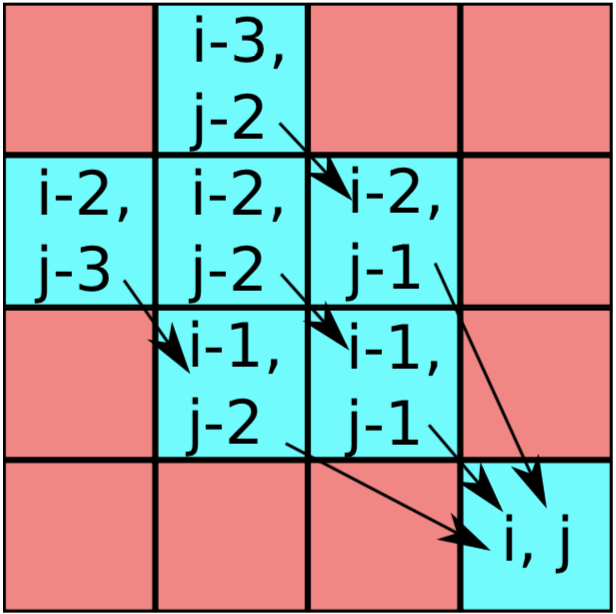
\includegraphics[height=4cm, keepaspectratio]{Algorithms/swworkings.png}
      \captionof{figure}[Smith-Waterman algorithm traversal]{SW algorithm traversal}
      \label{fig:swworkings}
    \end{minipage}%
    \begin{minipage}{.5\textwidth}
      \centering
      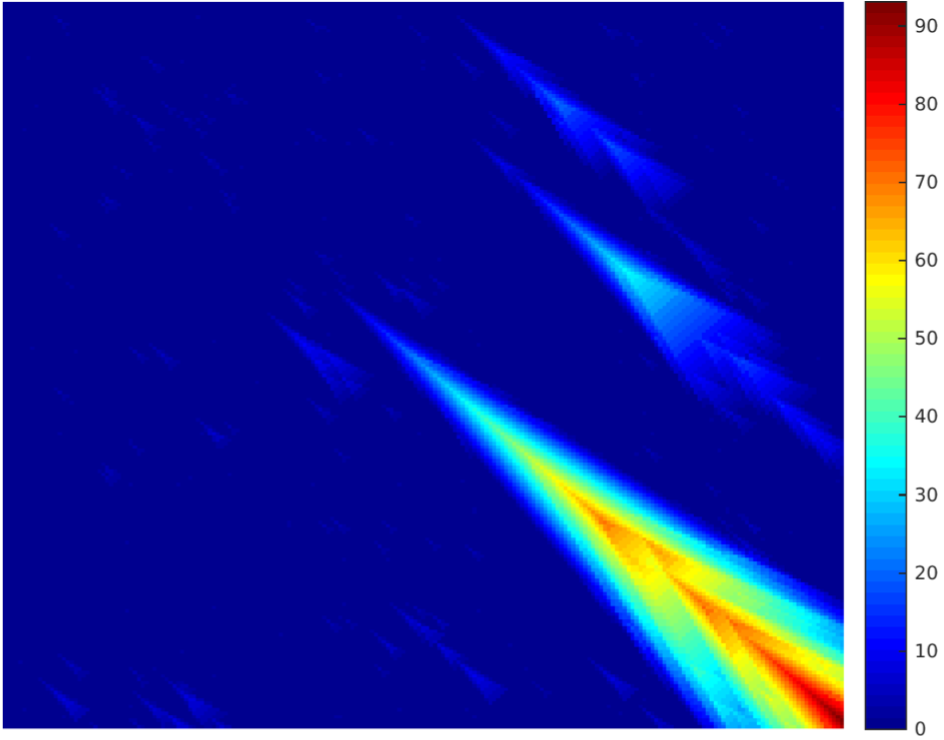
\includegraphics[height=5cm, keepaspectratio]{Algorithms/swmatrix.png}
      \captionof{figure}[Smith-Waterman matrix]{Smith-Waterman matrix displaying the scores calculated using equation \ref{eq:sw}}
      \label{fig:swmatrix}
    \end{minipage}
 \end{figure}

The finalised similarity score assigned after a run of the Smith-Waterman
algorithm is the sum of the scores along the longest identified local alignment.

\section{Aggregated rank rejector} 
\label{sec:rankaggregation}

Don't forget to mention that the 2DFT and other weak rejectors have not been
implemented due to lack of sufficient data

\section{Fingerprint rejector} 
\label{sec:rafii}

The final rejector examined is originally created to tackle the problem of live
song identification. It works on short query segments (usually from 6 to 10
seconds) or \textit{snippets} of live performance recordings. The sources of the
recordings vary from official live releases to amateur capturing of a live
performance through an audience-based device (smartphone, portable recorder,
etc.). The snippets are then compared to a song database through several image
processing techniques. It is the only analysed rejector which does not work with
full versions of songs.

\paragraph{}
As an initial step the rejector obtains frequency information using
\textit{Constant Q Transform (CQT)}. This technique, similarly to FFT,
transforms a signal from the time to frequency domain and produces a
spectrogram. While the frequency bins (the intervals of each frequency) in a FFT
spectrogram are uniformly spaced out, the bins resulting from CQT are
logarithmically spaced and follow the equal tempered scale. This is a better
representation of the human perception of frequencies. It also leads to a better
frequency resolution for the low and mid frequencies, as well as better time
resolution for high frequencies \cite{schorkhuber2010constant}.

The computation complexity of CQT is considerably high compared to FFT. The
exact implementation is not straight forward and it involves details beyond the
scope of my knowledge in the area. A further specification of CQT is therefore
unavailable in this report. In the benchmark a library implementation of CQT is
used throughout.

\paragraph{}
The first stage of the rejector is the \textit{fingerprinting stage}. After CQT
is applied on a song, the resulting spectrogram is converted into binary image
using adaptive thresholding. Threshold is a simple form of image segmentation
most frequently used to covert grayscale images into binary form. Thresholding
varies in relation to the type of image information used, adaptive thresholding
modifies each pixel value based on a local pixel neighbourhood of predetermined
size. For a neighbourhood around a pixel $(i, j)$ of matrix $X$ we calculate the
median of the neighbouring values:
\begin{equation}
   M(i, j) = median\; \{\; X(I, J) \mid i-\Delta_N \leq I \leq i+\Delta_N \text{ and } j-\Delta_N \leq J \leq j+\Delta_N \; \}
\end{equation}

In the median calculation $\Delta_N$ is the neighbourhood size. Using the local
median value the neighbourhood the point $X(i, j)$ can be binarised:
\begin{equation}
    B(i, j) = \begin{cases}
        1,& \text{if } X(i, j) > M(i, j) \\
        0,& \text{otherwise}
    \end{cases}
\end{equation}

By repeating the procedure for each element of the spectrogram we obtain the
binary matrix $B$. The ones in the representation indicate local areas with high
sound energy (the peaks of the spectrogram). A binary representation is
extracted for every song in the database. In the interest of clarity we refer to
the binary matrix of a database song as a \textit{reference fingerprint}. 

\begin{figure}[H]
   \centering
   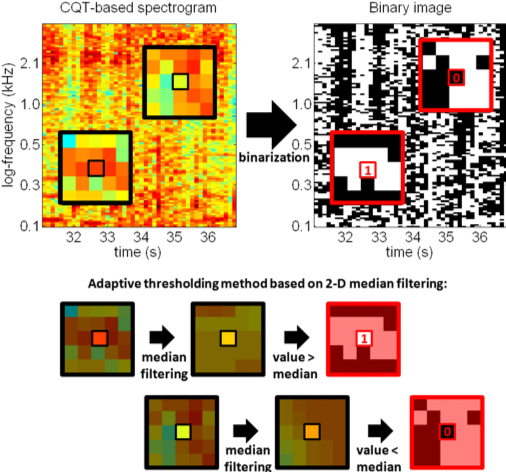
\includegraphics[width=0.7\textwidth]{Algorithms/adaptivethresh.png} 
   \captionof{figure}[Adaptive thresholding on CQT spectrogram]{Overview of the \textit{fingerprinting} stage of the rejector \cite{rafii2014audio}}
\end{figure}

The following \textit{matching} stage starts by constructing a similarity
matrices from the binary image of the query song and each of the reference
fingerprints. The similarity metric used is the Hamming similarity, i.e. the
percentage of values that match between both matrices. First, the reference
fingerprints are modified using the function $A(x) = 2x - 1$ and then multiplied
with the query fingerprint. The product is converted with the inverse of A
$(f_{-1} = (x + 1)/2)$. The resulting matrix is normalised by the frequency
dimension of the CQT spectrogram specification, which gives us a matrix
containing Hamming similarity scores for each pair of time frames between the
query segment and the reference.

After a further binarisation of the Hamming matrix using an empirically chosen
pre-defined fixed value, the final similarity score returned by the rejector is
calculated using the largest cumulated Hamming similarity defined by a line in
the matrix. A line containing the highest sum of similarity values signifies the
best alignment between a query segment and a reference fingerprint. Similarly to
the timbre rejector, because one of the dimensions represents alignment along
the time domain. Therefore the expected best alignment should correspond to a
diagonal line within the Hamming similarity matrix.

To detect best cumulative Hamming similarity in the matrix a method called
\textit{Hough transform} is utilised. The technique is a used to detect straight
lines within an image (or set of points) using the following line representation on a coordinate system:
\begin{equation}
   \rho = c \cos\theta + y \sin\theta
\end{equation}

where $\rho$ represents the shortest distance of the defined line from the
origin and $\theta$ is the angle between the $x$ axis and the perpendicular from
the origin to the line (figure \ref{fig:rthetaline}).

\begin{figure}[H]
    \centering
    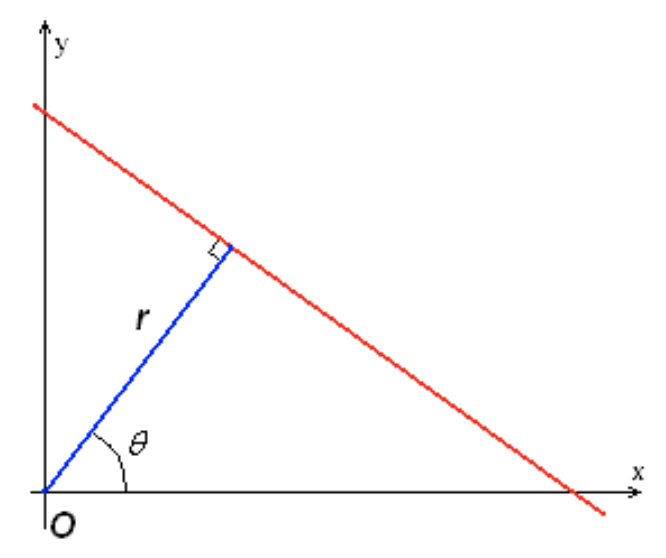
\includegraphics[width=0.4\textwidth]{Algorithms/rthetaline.png}
    \captionof{figure}[Hesse normal form of line]{Geometric representation of the Hesse normal form of a line}
    \label{fig:rthetaline}
\end{figure}

This equation helps us define a line using $(\rho, \theta)$. Plotting the set of
all values of $(\rho, \theta)$ for a fixed point describes a sine curve:

\begin{figure}[H]
   \centering
   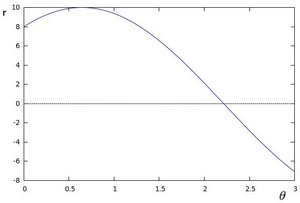
\includegraphics[width=0.4\textwidth]{Algorithms/houghlines.jpg} 
   \captionof{figure}[Sinusoidal curve of all lines within a point in relation to Hough transform]{Plot of the set of all lines through a single point}
\end{figure}

Given multiple points the straight line passing through all of them is
defined by the point in the $(\rho, \theta)$ plane which is the intersection of
all sinusoidal curves. Given a line the result of Hough transform is the set of
coordinates of the points lying on the line.

\paragraph{}
The fingerprint rejector exploits the idea of representing a line using a
distance and an angle. A range of values for $\rho$ and $\theta$ is defined and
the formed lines are passed to a Hough transform. The cumulative Hamming
similarity for the line is calculated using the locations within the matrix
returned by the transform.

\begin{figure}[H]
    \centering
    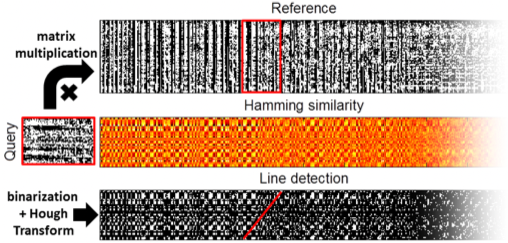
\includegraphics[width=0.6\textwidth]{Algorithms/matchingcqt.png}
    \label{fig:matchingcqt}
    \captionof{figure}[Matching phase of the fingerprint rejector]{Overview of the \textit{matching} phase of the rejector}
\end{figure}
